
% This first part of the document. Here you declare the type of document and the size of the text along with the paper size.
\documentclass[a4paper,11pt]{article}
%This is the packages used. They allow to use additional commands to format the document.
\usepackage[utf8]{inputenc}
\usepackage{graphicx}
\usepackage[english]{babel}
\usepackage[vmargin=3.5cm, top=2cm]{geometry}
\usepackage[linktocpage=true]{hyperref}
\usepackage{enumitem}
\usepackage{longtable}
\usepackage{pdfpages}
\usepackage{float}
\usepackage{hyperref}
\usepackage[section]{placeins}
\usepackage{listings}
\hypersetup{
    colorlinks,
    citecolor=black,
    filecolor=black,
    linkcolor=black,
    urlcolor=black
}
%New commands declared. This allows for easier declarations.
\newcommand{\tmtable}{\begin{longtable}{ p{2.7cm} p{10cm} }}
\newcommand{\tmtableend}{\end{longtable}}

\begin{document}
\lstset{language=C}  

%This is the titlepage. Here you can format and declare the front page of the document.
\begin{titlepage}
%Centers the text and removes automatic indentation
\centering \parindent=0pt
\newcommand{\HRule}{\rule{\textwidth}{1mm}}
\vspace*{\stretch{1}} \HRule\\[1cm]\large\bfseries
Title of the project\\[0.7cm]
\large Thesis Project\\[1cm]
\HRule\\[1cm]


\large by 
\\Mikkel Stolborg (msto@itu.dk)
\vspace*{\stretch{2}} \normalsize
\begin{flushleft}
IT University of Copenhagen \\
Supervisor\\
Name of supervisor\\
\today \end{flushleft}
\end{titlepage}

\begin{abstract}
Here you write the abstract of the project. The reason for having it as an abstract command section, is to not include it in the page count.
\end{abstract}
%breaks to next page.
\pagebreak
%Generates the table of content from the sections headings.
\tableofcontents
\pagebreak
\section{Install of latex}
In order to use and compile latex you need a latex compiler.

For a windows compiler go to: http://miktex.org/download

For a mac compiler go to: http://tug.org/mactex/

After you have a compiler, it is easier to work with latex in a latex editor, even though it can be done in any text editor. 

A great editor is TexMaker. It can be found here: http://www.xm1math.net/texmaker/
\section{Section}
A section is the top level of document. The structure goes section, subsection, and subsubsection.

The figure, a simple Image, can be referenced by its label. The figure \ref{fig:simpleImage}, will be the simple image.

\begin{figure}[h]
    \centering
    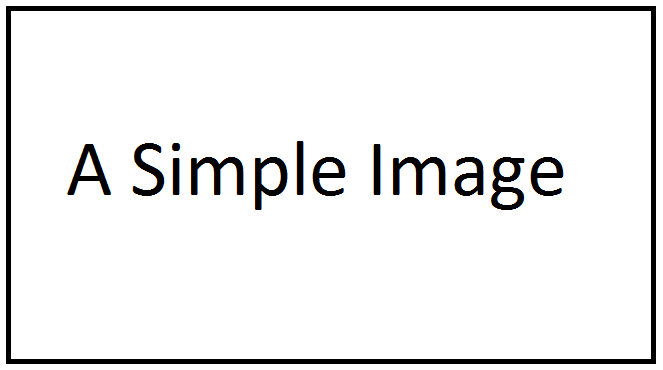
\includegraphics[width=0.8\textwidth]{Images/SimpleImage.png}
    \caption{This is the caption of the image. The figure is placed as close as possible to the text above. This is determined by the [h] command at the figure. The image is 80\% of the text width as given above. The image is located in a subfolder, as given in the path.}
    \label{fig:simpleImage}
\end{figure}

\subsection{Subsection}
\label{sec:subsection}
A subsection. you can reference to other sections by including a label beneath the section header.

In this section there is an equation. The equation \ref{func:function} is a simple linear function.
\begin{equation}
	y = \alpha \times x -\beta
	\label{func:function}
\end{equation}
\subsubsection{Subsubsection}
Here there is a reference to the section above. The section \ref{sec:subsection} is the over section above this sub subsection.

\begin{table}[h]
\centering
	\begin{tabular}{|c|l|r}
		% horizontal line, creates the lines in the table.
		\hline
		Center column & Left column & Right column\\ 
		\hline
		This is a table cell & This is another cell & so is this \\
		\hline
		There is no line & & \\
		between these cells & & \\		
		\hline
	\end{tabular}
	\caption{The selected tables data and selected columns}
	\label{Tab:simTab}
\end{table}

\section*{Hidden section}
This section does not appear in the table of contents. This is because of the star in the section declaration. Nor does a number appear next to the section header.
\subsection*{Hidden subsection}
The star can be applied to all levels of sections.
\subsubsection*{Hidden subsubsection}
This hidden style can be used as small headings, without adding it to the table of contents.

\section{Other notes}
It is possible to do much more than described here, and usually you can simple google want you want to do, followed by Latex. That will usually give you a quick guide.
\subsection{Importing latex files}
It is possible to import other latex files into a main file. For our purpose we will have other latex files imported using the \textbackslash include command.


\begin{thebibliography}{1}

\bibitem{bibitemName}
Author 1, Author 2, and Author 3, \emph{Title of article or book}, Place of print and or writing, publishing year.
\bibitem{experience}
Georgios N. Yannakakis and Julian Togelius, \emph{Experience-Driven Procedural Content Generation}, Member, IEEE, 2011.
\end{thebibliography}



\end{document}
